\documentclass[a4paper,12pt]{report}

\usepackage{cmap}
\usepackage[T2A]{fontenc}
\usepackage[utf8]{inputenc}
\usepackage[russian]{babel}
\usepackage{amsmath,amsfonts,amssymb}
\usepackage{graphicx}
\usepackage{sidecap}
\usepackage{wrapfig}
\usepackage{indentfirst}

\begin{document} 

\begin{titlepage} 

\begin{center} 

\large Федеральное государственное автономное образовательное учреждение высшего образования «Санкт-Петербургский государственный электротехнический университет «ЛЭТИ» им. В.И. Ульянова (Ленина)»\\
кафедра Вычислительной техники\\[5cm] 

\huge ОТЧЕТ\\ по лабораторной работе № 11\\[0.5cm] 
\large <<Битовые поля в структурах>>\\[3.7cm]

\begin{minipage}{1\textwidth}
    \begin{flushleft}
        \emph{Автор:} Стукен В.А.\\
        \emph{Группа:} 2307\\
        \emph{Факультет:} ФКТИ\\
        \emph{Преподаватель:} Аббас Саддам Ахмед\\
    \end{flushleft}
\end{minipage}

\vfill

Санкт-Петербург, 2023\\
{\large \LaTeX}

\end{center}
\thispagestyle{empty}
\end{titlepage}

\section*{Задание(вариант 11)}

Числовой адрес компьютера в глобальной сети Интернет (ip-адрес) версии 4 состоит из 4-х чисел от 0 до 255, разделенных точками (например, 123.45.67.89). Для записи каждого числа используется 1 байт (октет). Значения первого числа ip-адреса определяют т. н. «класс сети»\\ 

Поскольку адресов IPv4 недостаточно, используются т. н. «частные сети», адреса которых могут повторяться в различных изолированных локальных сетях.

Адреса «частных сетей» класса C всегда начинаются с 192, а вторым числом всегда является 168 (например, 192.168.234.77)

Разработать алгоритм и реализовать функции преобразования произвольного адреса IPv4 в адрес «частной сети» класса C с использованием битовых полей в структурах и битовых операций.

\section*{Постановка задачи и описание решения}
\par

Задаем структуру, состоящую из четырех полей типа unsingned int размером 8 бит. В таком случае максимальное число, которое возможно будет записать в это поле - 255. Далее пользователь вводит Ip-адрес, мы задаем полям структуры соответствующие значения. Затем с помощью битовых операций меняем первые два числа на 192 и 168 соответственно. Выводим преобразованный IP-адрес.
\section*{Описание переменных-функция main}
\begin{centering}
\resizebox{14cm}{!}{
    \begin{tabular}{|l|l|l|l|}
        \hline
        \textbf{№} & \textbf{Имя переменной} & \textbf{Тип} & \textbf{Назначение}\\
        \hline
        1 &  first   &  int & Первый октет IP-адреса \\
        \hline
        2 &  second   &  int & Второй октет IP-адреса \\
        \hline
        3 &  third   &  int & Третий октет IP-адреса \\
        \hline
        4 &  fourth   &  int & Четвертый октет IP-адреса \\
        \hline
        5 &  ip   &  IPN & Структура IP-адреса \\
        \hline
        
        
    \end{tabular}
}
\end{centering}
\section*{Примеры работы программы:}
\begin{figure}[ph]
    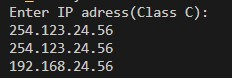
\includegraphics[width=0.7\textwidth]{ex1.jpg}
\caption{Пример 1}
\label{ris:image1}
\end{figure}
\begin{figure}[ph]
    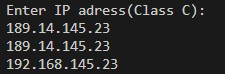
\includegraphics[width=0.7\textwidth]{ex2.jpg}
\caption{Пример 2}
\label{ris:image2}
\end{figure}




\begin{figure}[ph]
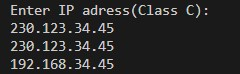
\includegraphics[width=0.7\textwidth]{ex3.jpg}
\caption{Пример 3}


\end{figure}


\newpage

\section*{Вывод}
В данной лабораторной работе использовали битовые поля в структурах, а также битовые операции.

\end{document}